%%%%%%%%%%%%%%%%%%%%%%%%%%%%%%%%%%%%%%%%%%%%%%%%
%
% == AIT CSIM Handout LaTeX Template ==
% == Credit ==
% Assoc. Prof. Matthew N. Dailey
% Computer Science and Information Management
% Asian Insitute of Technology
%
%%%%%%%%%%%%%%%%%%%%%%%%%%%%%%%%%%%%%%%%%%%%%%%%

\documentclass{article}

\usepackage{a4, url, upquote}
\usepackage{graphicx}
\usepackage{hyperref}
\usepackage[cmex10]{amsmath}
\usepackage{amssymb}
\usepackage{placeins}
\usepackage{listings}

\setlength{\textwidth}{6.5in}
\setlength{\textheight}{9in}
\setlength{\oddsidemargin}{0in}
\setlength{\evensidemargin}{0in}
\setlength{\topmargin}{0in}
\setlength{\headheight}{0in}
\setlength{\headsep}{0in}
\setlength{\footskip}{0.5in}

\newcommand{\bheading}[1]{\vspace{10pt} \noindent \textbf{#1}}

\begin{document}

\begin{tabbing}
    \`\=\kill
    \textbf{Workshop:} The WordPress Way
    \` September 11, 2015 \\
    \textbf{Instructor:} Kan Ouivirach ({\tt \small kan@prontomarketing.com})
        and Navarant Pramuksan ({\tt \small oy@prontomarketing.com}) \\
    \textbf{Company:} Pronto Marketing (Research and Develpment Team)
\end{tabbing}

\hrule

\vspace{.25in}

\begin{center}
    \textbf{\Large The WordPress Way: Customizing WordPress Theme and
        Developing WordPress Plugins}
\end{center}

\vspace{.15in}

\noindent \textbf{Introduction:} This workshop is intended for anyone who wants
to learn WordPress and do things the WordPress way. Participants will learn how
to customize a WordPress theme and better understand how WordPress template
hierarchy works. Participants will also learn how to develop a WordPress plugin
to enhance the funtionality of the theme. By the end of this workshop,
participants will be able to develop their own WordPress theme and use
WordPress as a solution to real-world problems.

\section*{Customizing WordPress Theme}

\noindent In this section, we will customize a WordPress theme
``ThirtyFifteen'' and follow the WordPress template hierarchy~[1] to extend a
new template for a new custom post type. Let's get started. \\

\noindent We are going to duplicate the ThirtyFifteen theme and rename it to
TheWordPressWay. Doing this way allows us to keep the originial theme
unmodified and redo this workshop as many times as we want.

\begin{enumerate}
    \item Go to the directory {\tt wp-content/themes/}.
    \item Duplicate the directory {\tt twentyfifteen} and rename it
        to {\tt thewordpressway}.
    \item Open the file {\tt style.css}, remove the current settings in the
        comments, and use these settings below:
        \begin{itemize}
            \item[-] Theme Name: The WordPress Way
            \item[-] Author: Kan Ouivirach
            \item[-] License: MIT
        \end{itemize}
    \item Go to your WordPress site and change the theme to The WordPress Way.
\end{enumerate}

\noindent Right now we should have The WordPress Way theme activated as seen in
Figure~\ref{fig:fig:activating-custom-theme}. Next we are going to make some
simple change on a very simple template. Here the template like 404 page is a
good start.

\FloatBarrier

\begin{figure}[t]
    \centering
    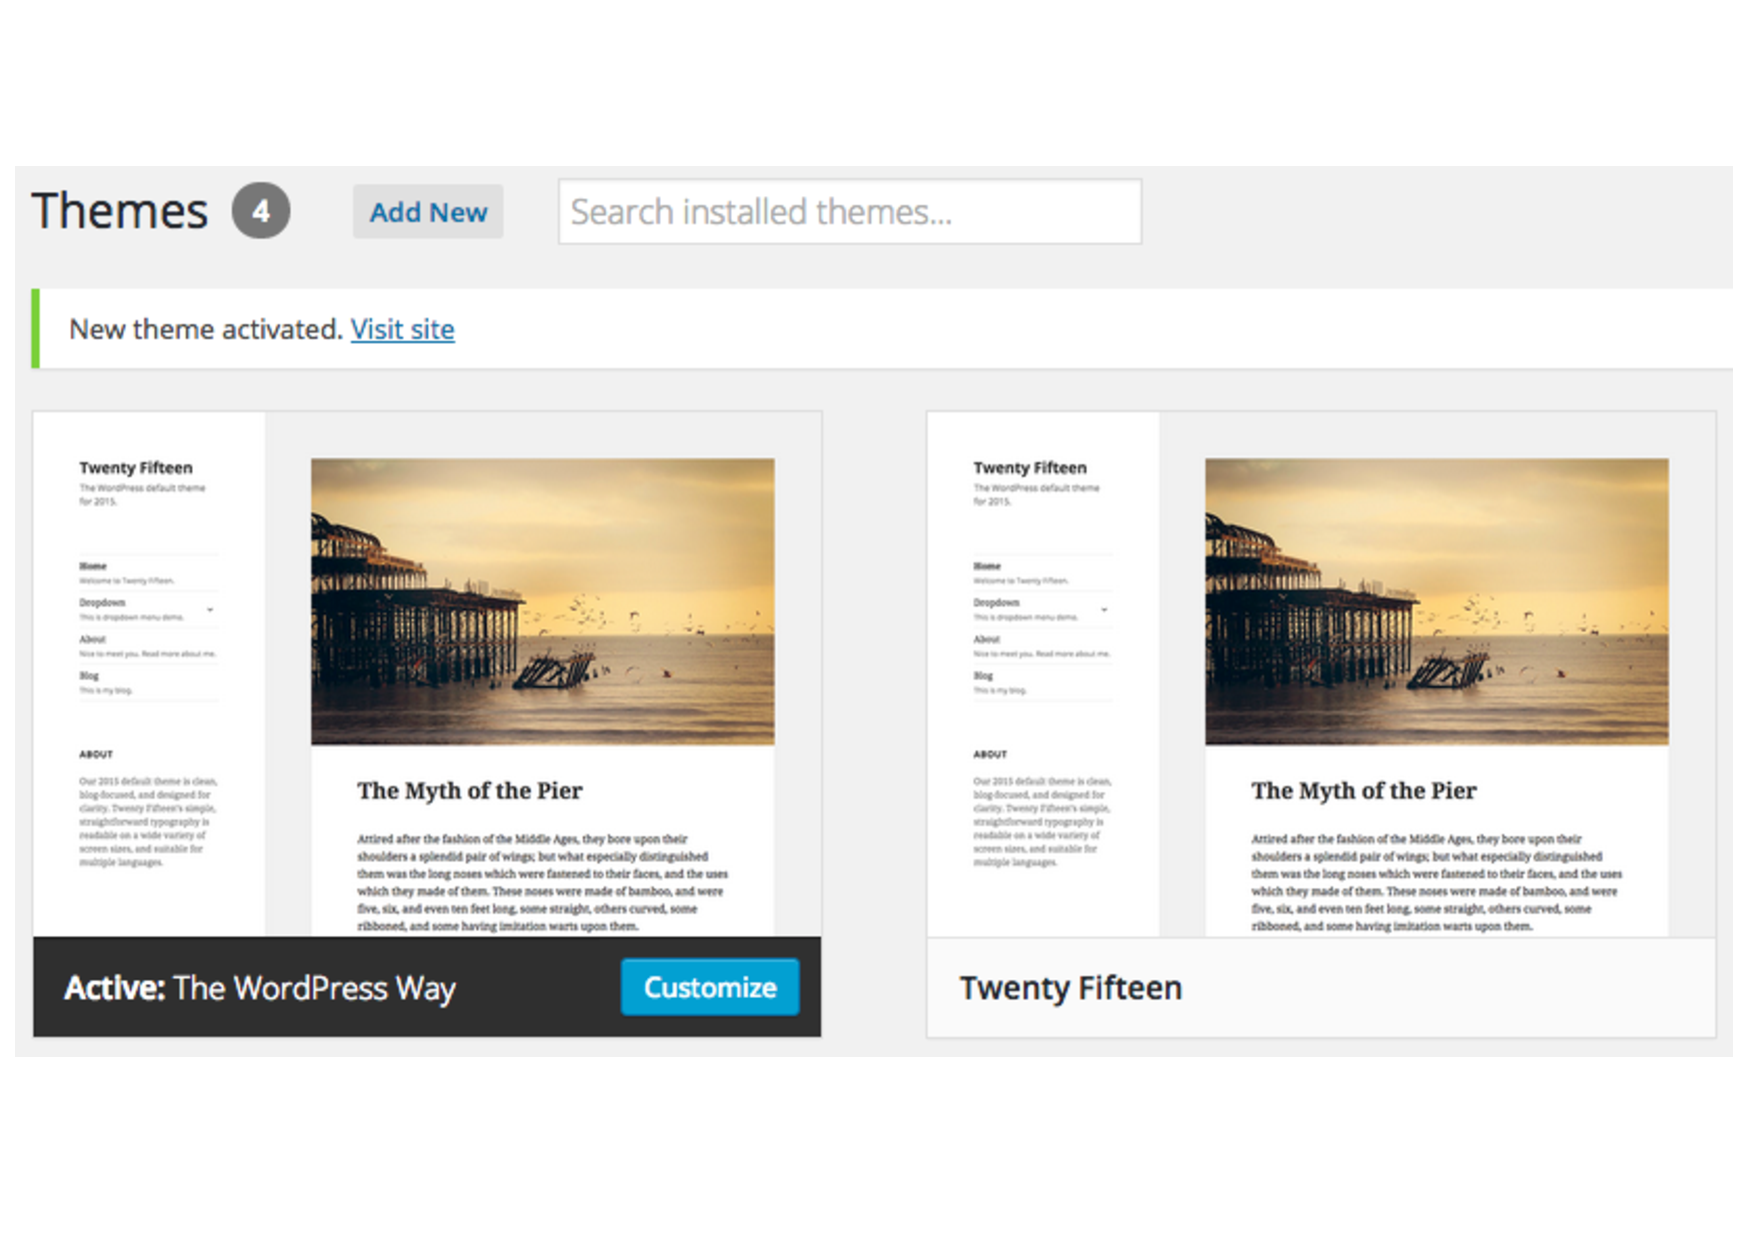
\includegraphics[width=4in]{figures/activating-custom-theme}
    \caption{Activating a Custom Theme}
    \label{fig:activating-custom-theme}
\end{figure}

\begin{enumerate}
    \item Go to your theme directory {\tt wp-content/themes/thewordpressway}.
    \item Open the file {\tt 404.php}.
    \item Let's make it more attractive. Find any image from the Internet and
        put it somewhere on the page. Don't forget to put a credit if the
        image is not yours.
    \item When we access a non-existing page such as
        {\tt http://localhost/?p=99999}, we should see our nice custom
        404 page.
\end{enumerate}

\noindent Your 404 page should look similar to the one shown in
Figure~\ref{fig:custom-404-page}. Below is the code that does that.

\begin{verbatim}
<div id="primary" class="content-area">
  <main id="main" class="site-main" role="main">
    <section class="error-404 not-found">
      <header class="page-header">
        <h1 class="page-title">Oops! Sorry, this page doesn't exist.</h1>
      </header>
      <div class="page-content">
        <p style="text-align: center;">
          <img src="<?php echo get_template_directory_uri(); ?>/images/molodotme.jpg">
        </p>
        <p style="text-align: center;">
          <strong>Credit:</strong> <a href="http://molome.com/" target="_blank">MOLOME</a>
        </p>
        <?php get_search_form(); ?>
      </div>
    </section>
  <main>
</div>
\end{verbatim}

\begin{figure}[t]
    \centering
    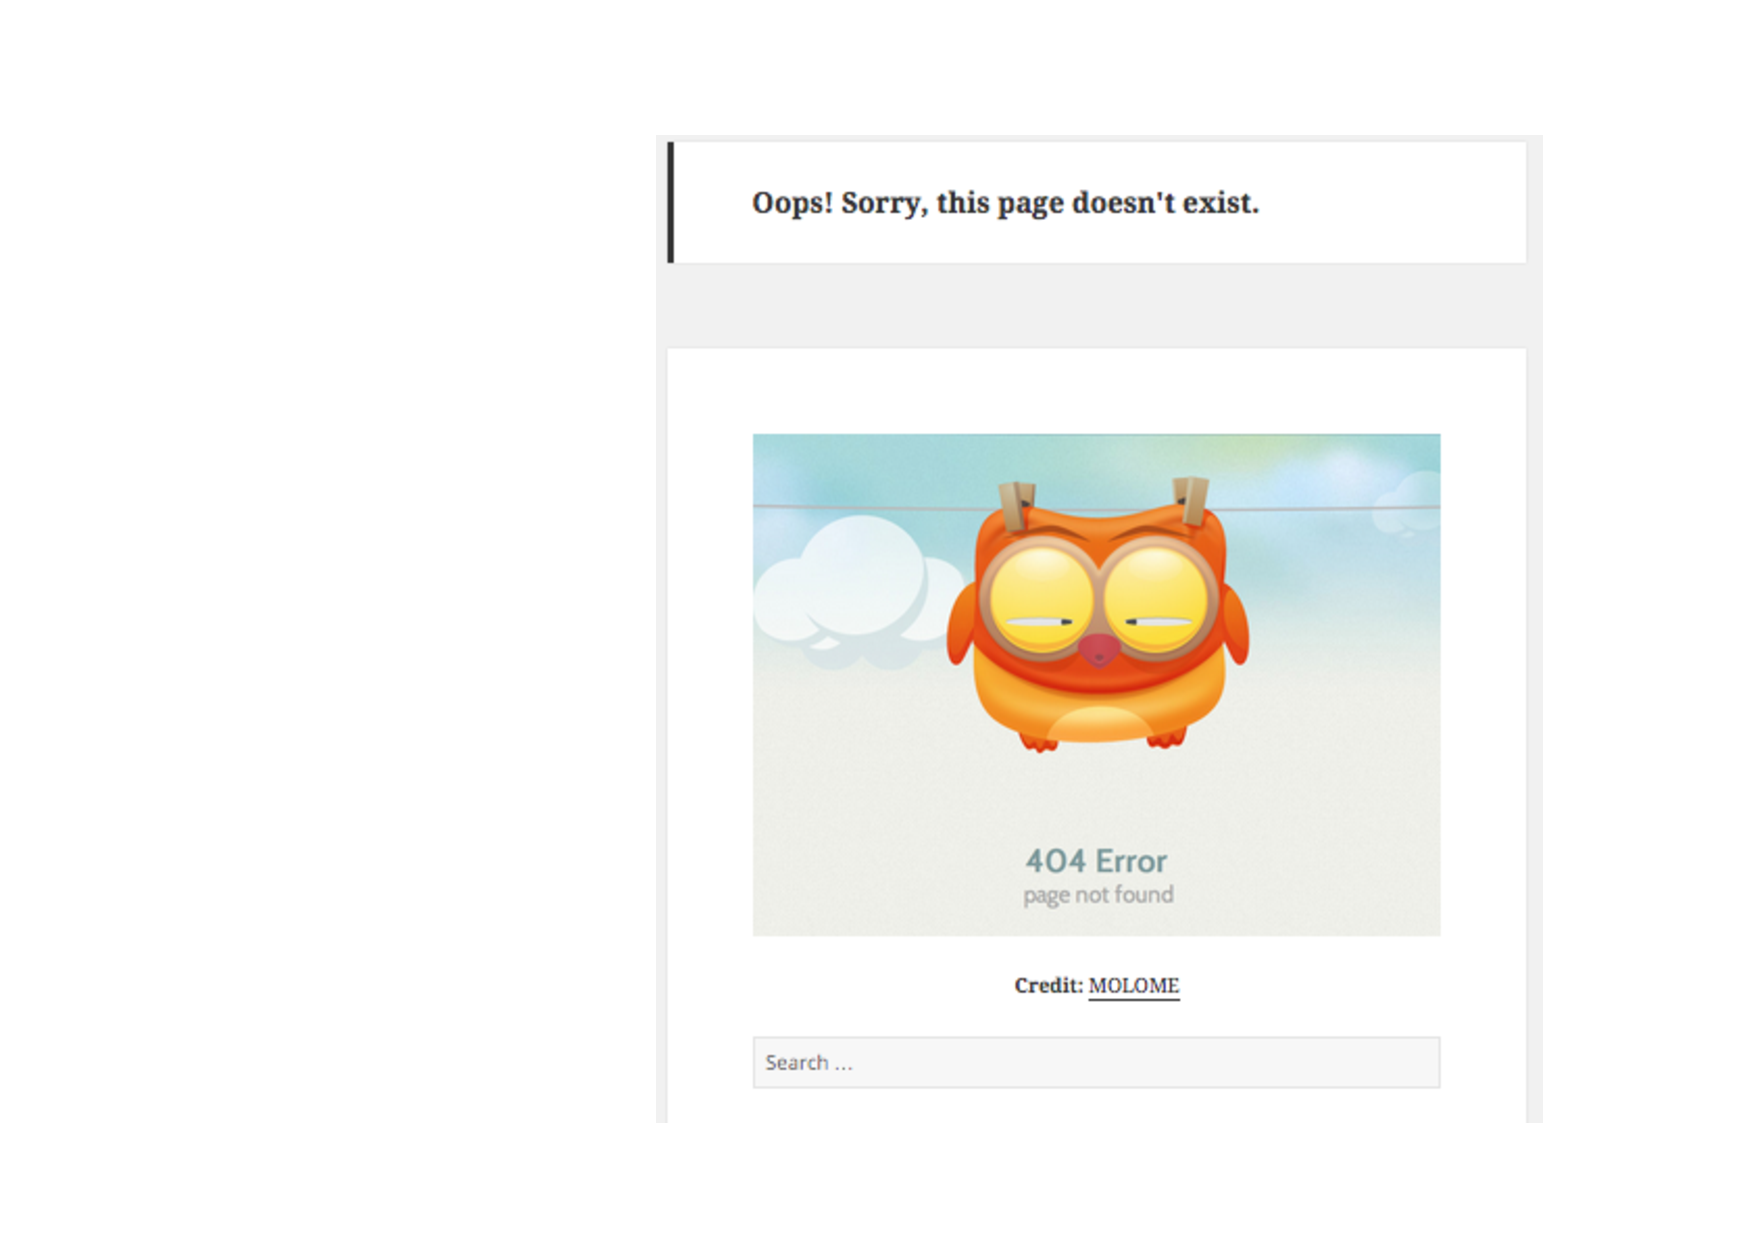
\includegraphics[width=3in]{figures/custom-404-page}
    \caption{Custom 404 Page}
    \label{fig:custom-404-page}
\end{figure}

\noindent Great work! Now you have an experience on customizing the WordPress
template. You can upgrade yourself to the next level, extending the template.
\\

\noindent {\bf Challenge:} Let's look at the WordPress template hierarchy for a
minute. Suppose we have our own custom post type and want to create a template
for it. What should we do to accomplish this task? \\

\noindent {\bf Hint:} Look at the WordPress template hierarchy and read Post
Type Template~[2].

\section*{Developing WordPress Plugin}

\noindent In this section, we will create a simple plugin called My Awesome
Team. The scenario is that you want to show how awesome your team is by listing
your teammates on your WordPress site. You also want to be able to click on
your teammate's name and see his/her brief information. Let's get your hand
dirty! \\

\noindent Create the plugin by following these steps below.

\begin{enumerate}
    \item Create a new directory {\tt my-awesome-team} under the directory {\tt
        wp-content/plugins}.
    \item Create a new file {\tt my-awesome-team.php} under the new directory
        {\tt my-awesome-team} and place the code below
\begin{verbatim}
<?php
/*
 * Plugin Name: My Awesome Team
 * Description: A plugin to list my awesome teammates
 * Author: Kan Ouivirach
 */
\end{verbatim}
    \item Go to the Plugins page. If you have done it correctly, your plugin
        will be listed as shown in Figure~\ref{fig:my-awesome-team-plugin}.
\end{enumerate}

\begin{figure}[t]
    \centering
    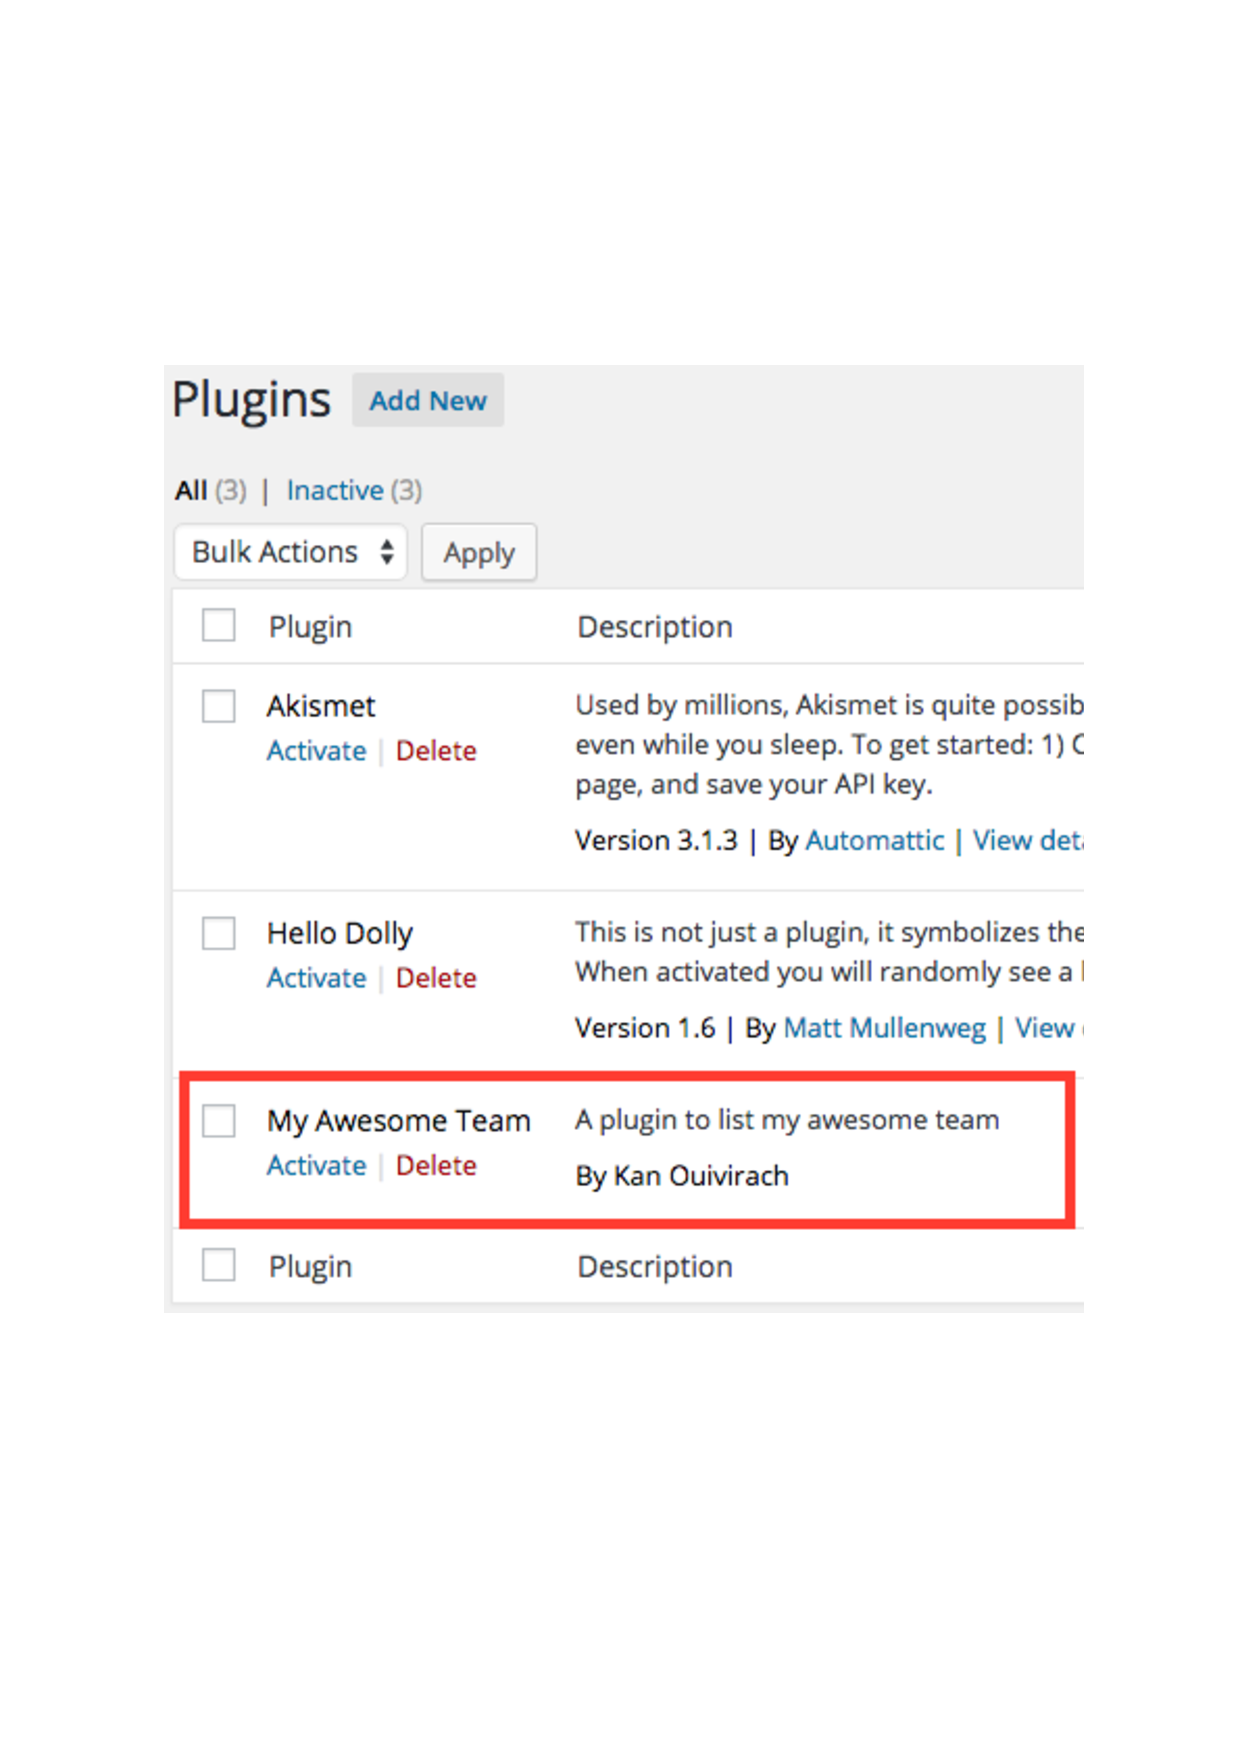
\includegraphics[width=3in]{figures/my-awesome-team-plugin}
    \caption{My Awesome Team Plugin}
    \label{fig:my-awesome-team-plugin}
\end{figure}

\noindent Next we are going to register the teammate custom post type since we
would like to keep our teammate information in the database. For more
information on registering a custom post type, see Register Post Type~[3].
Below is the code for registering our custom post type.

\begin{verbatim}
function teammate_setup_post_type() {
  $labels = array(
    'name'          => __( 'Teammates' ),
    'singular_name' => __( 'Teammate' ),
    'add_new'       => __( 'Add New' ),
    'add_new_item'  => __( 'Add New Teammate' ),
    'edit_item'     => __( 'Edit Teammate' ),
    'new_item'      => __( 'New Teammate' ),
    'all_items'     => __( 'All Teammate' ),
    'view_item'     => __( 'View Teammate' ),
    'search_items'  => __( 'Search Teammate' ),
    'not_found'     => __( 'No Teammate Found' )
  );

  $args = array(
    'labels'             => $labels,
    'description'        => 'Teammate involved in attempting to achieve a common goal.',
    'public'             => true,
    'publicly_queryable' => true,
    'has_archive'        => true,
    'capability_type'    => 'page',
    'show_ui'            => true,
    'hierarchical'       => false,
    'query_var'          => true,
    'supports'           => array(
      'title',
      'editor',
      'thumbnail'
    ),
    'show_in_nav_menus'  => false,
  );
  register_post_type( 'teammate', $args );
}
add_action( 'init', 'teammate_setup_post_type', 10 );
\end{verbatim}

\noindent If you have done this correctly, the teammate menu should be listed
in the site as shown in Figure~\ref{fig:teammate-menu}. That's it! Now we can
save our teammate information in the database. Simple, right? :-) \\

\begin{figure}[t]
    \centering
    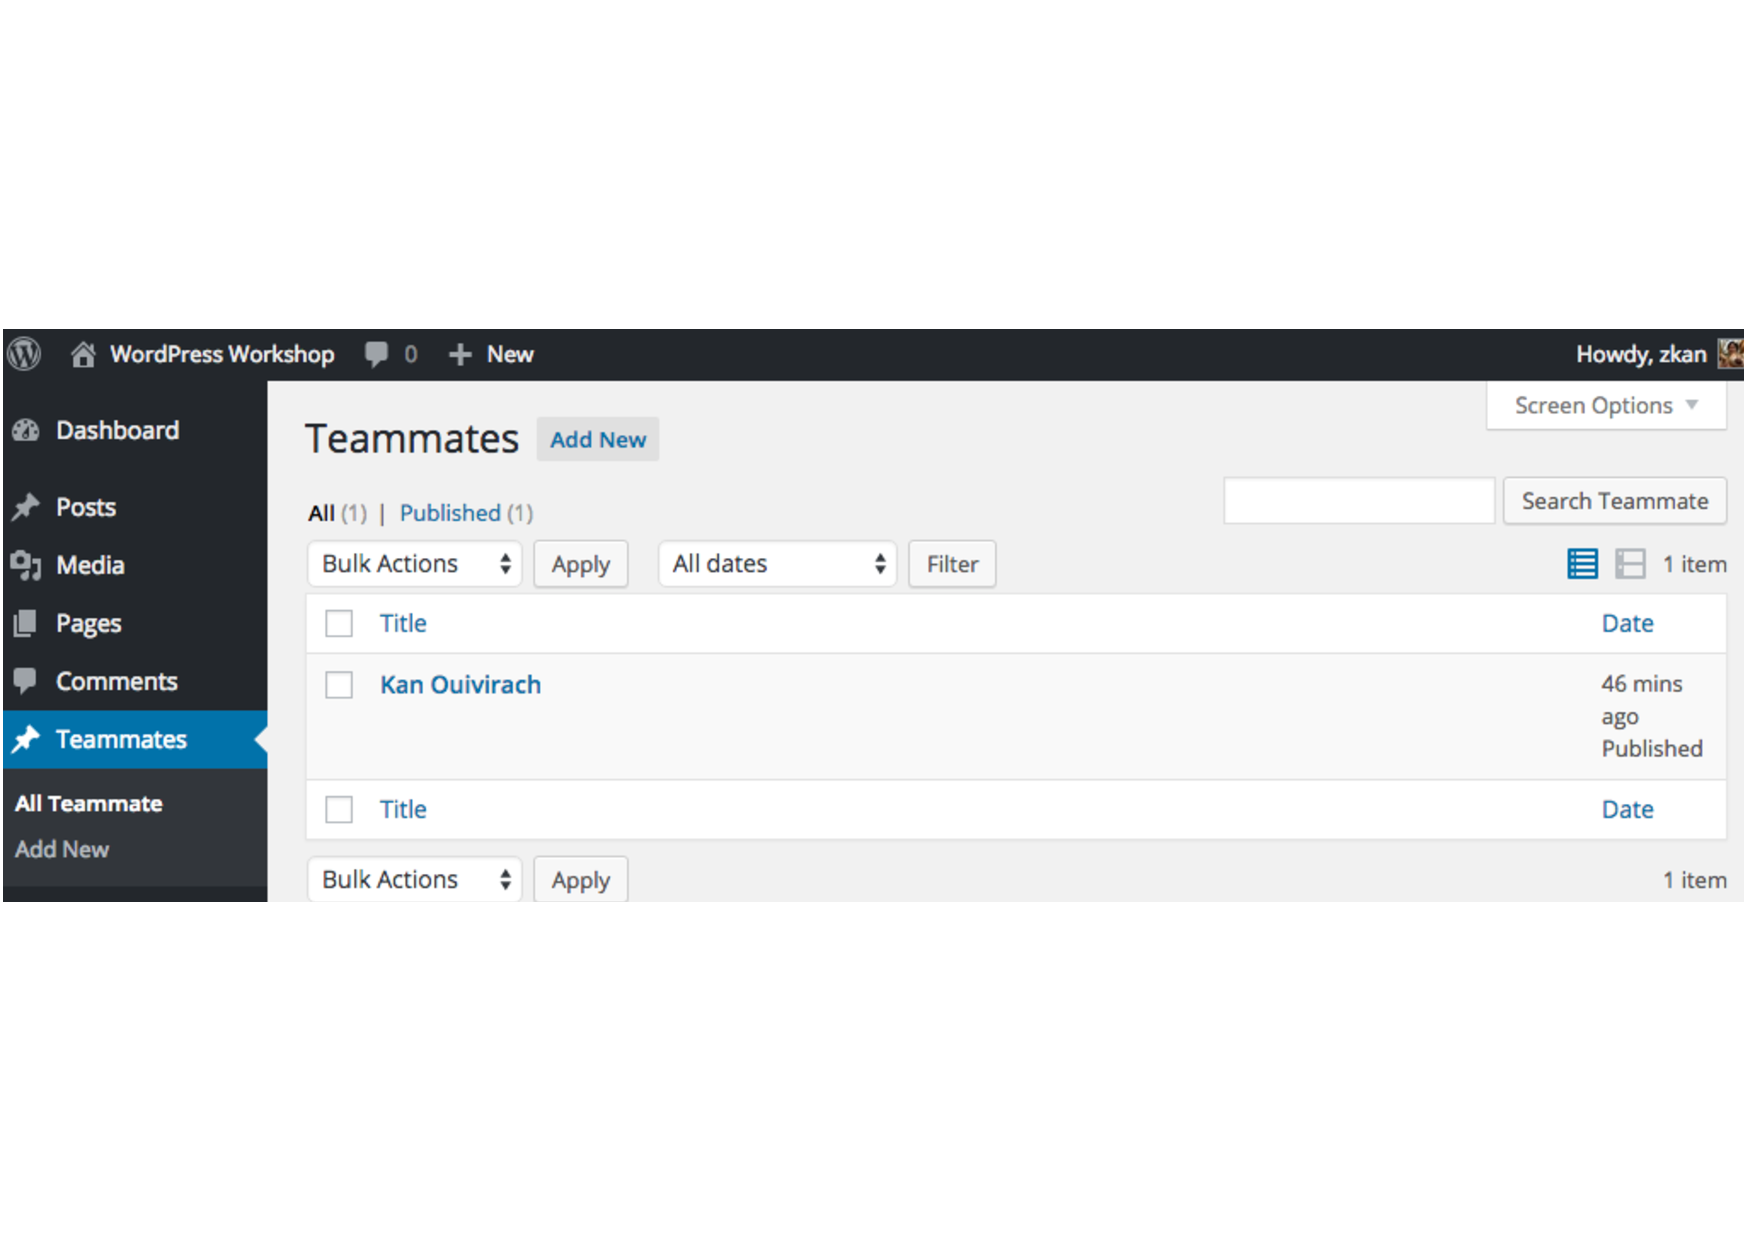
\includegraphics[width=6in]{figures/teammate-menu}
    \caption{Teammate Menu}
    \label{fig:teammate-menu}
\end{figure}

\noindent Our work is not done yet. We need to show our awesome teammates on
the site, so let's create a page to show them. One way to do this is to
manually put the information on the page with the code below. Don't forget to
switch to the Text mode before place the code. Figure~\ref{fig:teammate-list}
shows the result from the code.

\begin{verbatim}
<h4><a href="#" onClick="teammate_toggle('teammate_1')">Kan Ouivirach</a></h4>
<p id="teammate_1" style="display: none;">Instructor</p>
<h4><a href="#" onClick="teammate_toggle('teammate_2')">Navarat Pramuksan</a></h4>
<p id="teammate_2" style="display: none;">Teaching Assistant</p>

<script type="text/javascript">
function teammate_toggle(id) {
  var element = document.getElementById(id);
  element.style.display = ((element.style.display != 'none') ? 'none' : 'block');
}
</script>
\end{verbatim}

\begin{figure}[t]
    \centering
    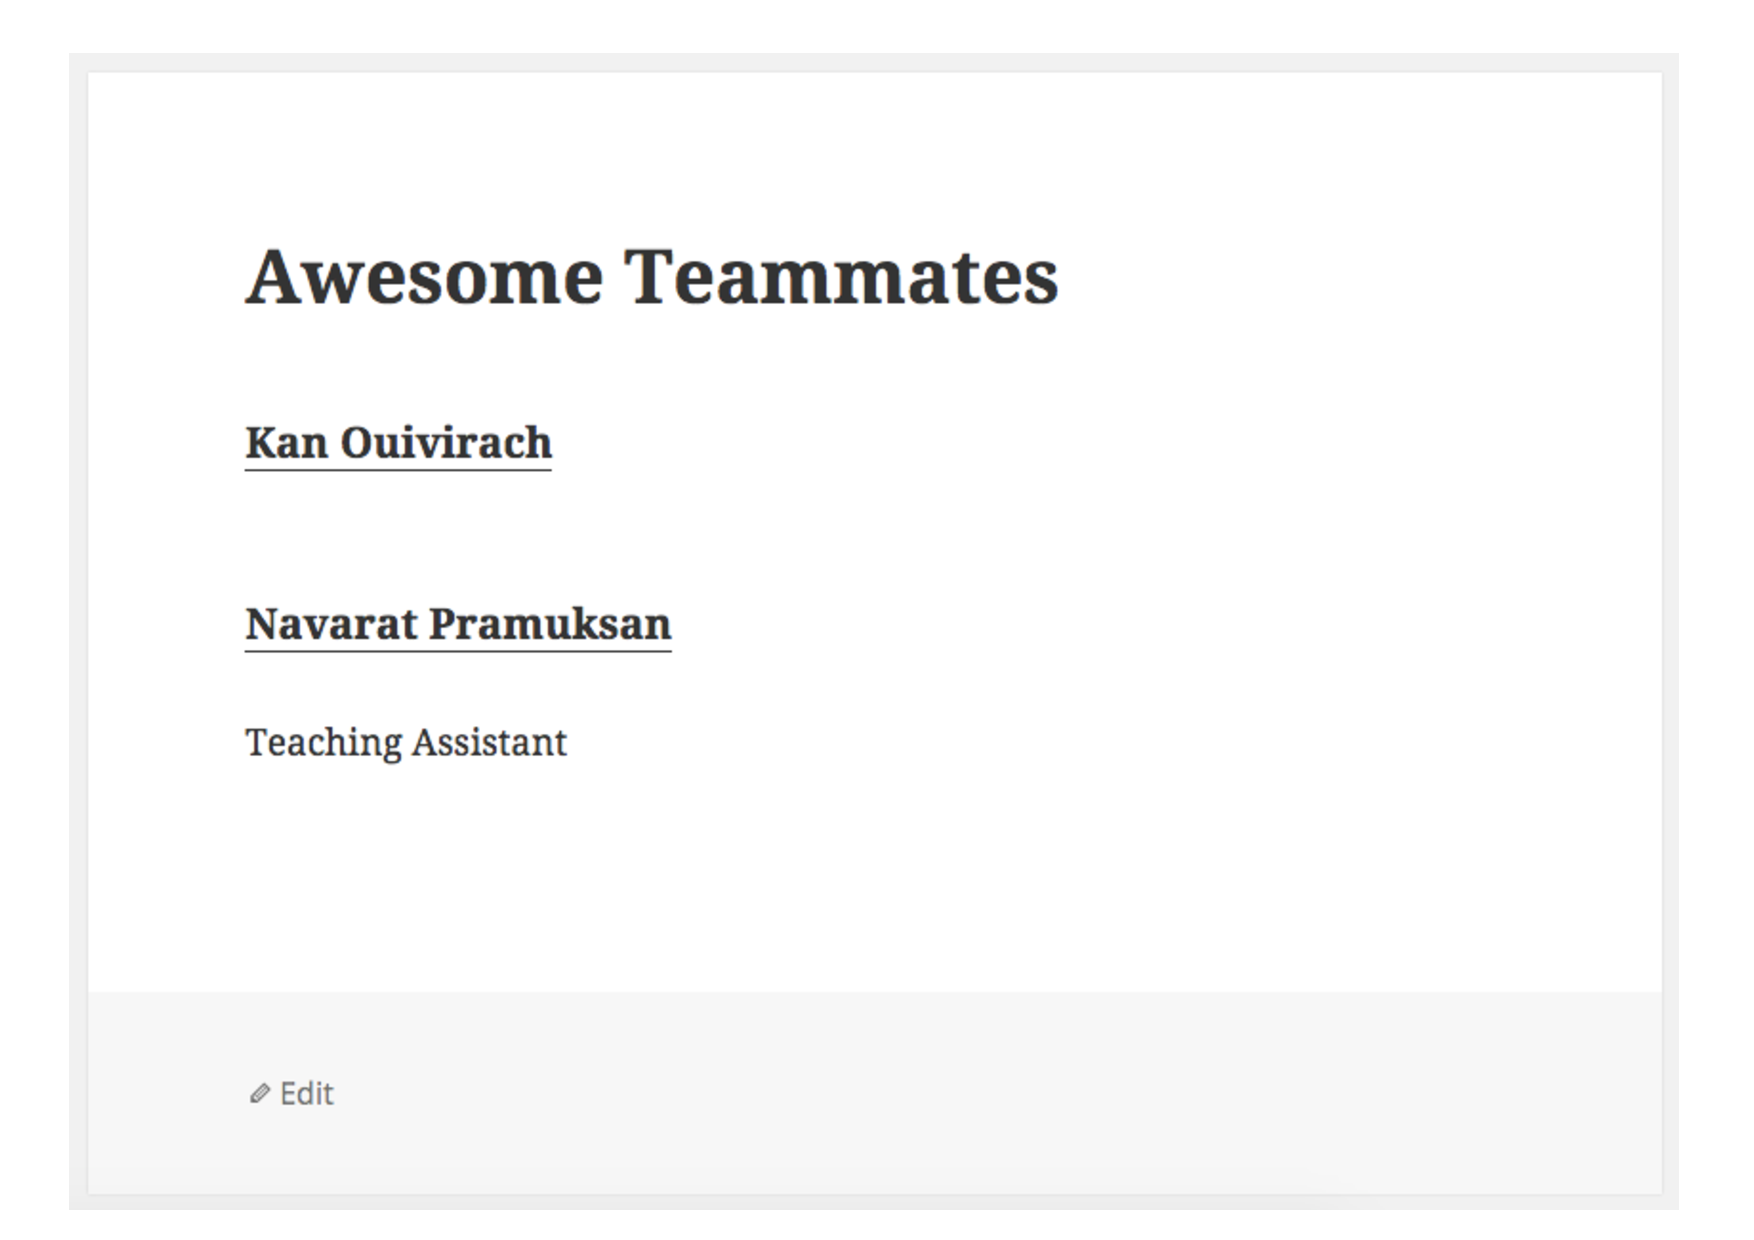
\includegraphics[width=4in]{figures/teammate-list}
    \caption{Teammate List}
    \label{fig:teammate-list}
\end{figure}

\noindent However, this way is not convenient for us to maintain our teammate
list. The better way is to use the shortcode API~[4], which is a nice feature
that enables us to generate content without inserting any HTML code. Let's
build one! Open our plugin file {\tt my-awesome-team.php} and place the code
below.

\begin{verbatim}
function teammate_shortcode( $atts ) {
  $args = array(
    'post_type' => 'teammate',
    'order'     => 'ASC'
  );

  $html = '';

  $posts = get_posts( $args );
  foreach ( $posts as $post ) {
    $html .= '<h4><a href="#" onClick=\'teammate_toggle("teammate_';
    $html .= $post->ID;
    $html .= '")\'>';
    $html .= $post->post_title;
    $html .= '</a></h4>';
    $html .= '<p id="teammate_';
    $html .= $post->ID;
    $html .= '" style="display: none;">';
    $html .= $post->post_content;
    $html .= '</p>';
  }

  $html .= '<script type="text/javascript">';
  $html .= 'function teammate_toggle(id) {';
  $html .= 'var element = document.getElementById(id);';
  $html .= 'element.style.display = ((element.style.display != "none") ? "none" : "block");';
  $html .= '}';
  $html .= '</script>';

  return $html;
}
add_shortcode( 'teammate', 'teammate_shortcode' );
\end{verbatim}

\noindent What we just did is that we created a function to query the posts of
which post type is {\tt teammate} and constructed the HTML and return it. At
the end, we registered our function to the shortcode {\tt teammate}. \\

\noindent Right now we can go back to edit the page and just put {\tt
[teammate]} in the content. If we have done it correcly, we should have the
result the same as shown in Figure~\ref{fig:teammate-list}. Well done! \\

\noindent What if we want to limit the number of teammates to show? We can do
that by allowing our shortcode to take parameters. WordPress has a nice
function we can use called {\tt shortcode\_atts}~[4]. The description from
Shortcode API~[5] says:

\begin{quote}
Combines user shortcode attributes with known attributes and fills in defaults
when needed. The result will contain every key from the known attributes,
merged with values from shortcode attributes.
\end{quote}

\noindent We can modify our code before we define the arguments for the
function {\tt get\_posts} as follows.

\begin{verbatim}
$defined_atts = array(
  'limit' => -1,
);
extract( shortcode_atts( $defined_atts, $atts ) );

if ( $limit ) {
    $posts_per_page = $limit;
}

$args = array(
  'posts_per_page' => $posts_per_page,
  'post_type'      => 'teammate',
  'order'          => 'ASC'
);
\end{verbatim}

\noindent Go back to edit the page. Change {\tt [teammate]} to {\tt [teammate
limit=1]} and see what happens. Try to play around with it. :-) \\

\noindent {\bf Challenge:} It is not so nice to render the JavaScript code
along with the HTML we generate. It would be better if we can refactor it. \\

\noindent {\bf Hint:} Look at the function {\tt wp\_enqueue\_script}~[6].

\section*{References}

\begin{itemize}
    \item[1] WordPress Template Hierarchy -- {\tt http://wphierarchy.com/}
    \item[2] Post Type Template -- {\tt http://codex.wordpress.org/Post\_Type\_Templates}
    \item[3] Register Post Type -- {\tt http://codex.wordpress.org/Function\_Reference/register\_post\_type}
    \item[4] Function {\tt shortcode\_atts} -- {\tt https://codex.wordpress.org/Function\_Reference/shortcode\_atts}
    \item[5] Shortcode API -- {\tt https://codex.wordpress.org/Shortcode\_API}
    \item[6] Function {\tt wp\_enqueue\_script} -- {\tt https://codex.wordpress.org/Function\_Reference/wp\_enqueue\_script}
\end{itemize}

\end{document}
